\documentclass{article}
\usepackage[utf8]{inputenc}

\usepackage{amssymb}
\usepackage{amsmath}

\title{Time Series Project 1}
\author{Stefan Eng and Franz Hartleitner}
\date{April 2019}

\usepackage{natbib}
\usepackage{graphicx}

\begin{document}

\maketitle

\section*{Problem 1}

\begin{figure}[h!]
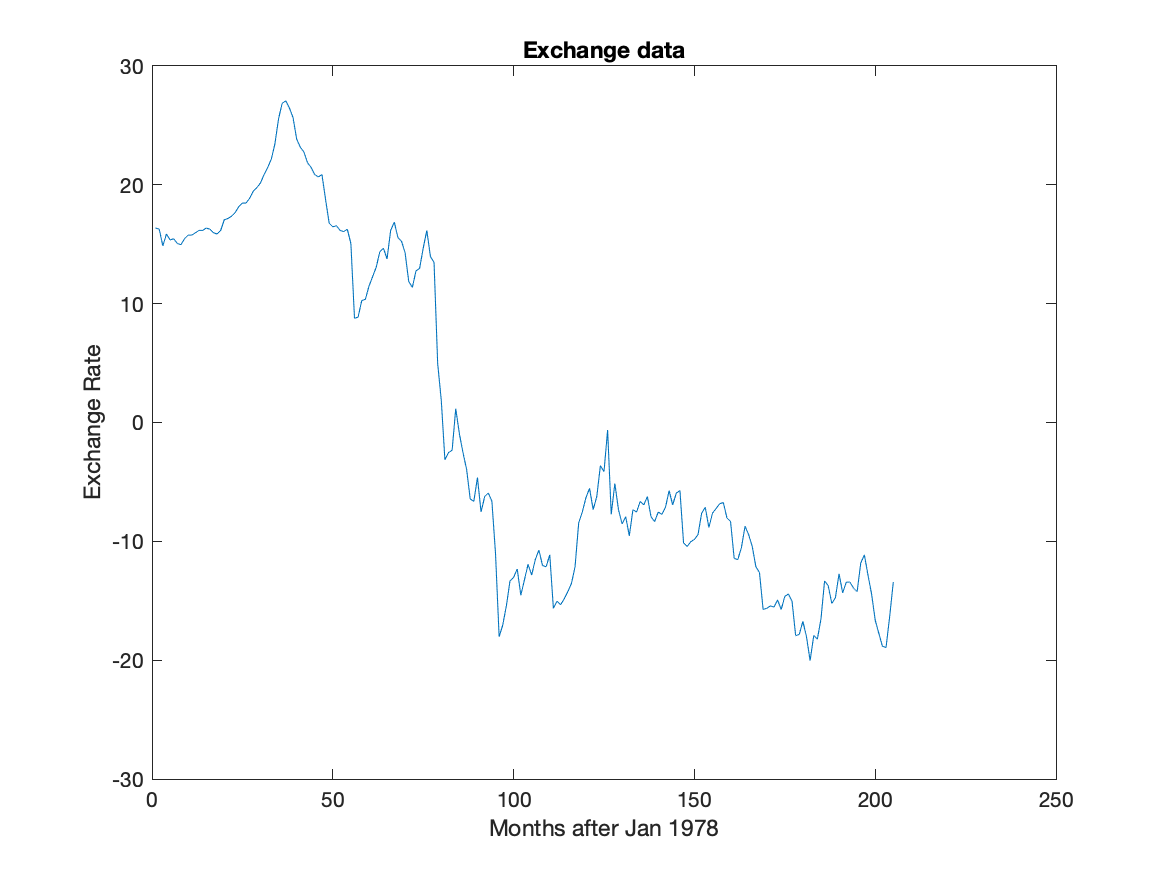
\includegraphics[width=10cm]{plots/exchangedata.png}
\centering
\caption{Monthly observations of the Australian Trade Weighted Index}
\label{fig:exchangerate}
\end{figure}

In Figure \ref{fig:exchangerate} we we can see the the monthly observations of the Australian Trade Weighted Index.
From this graph it does not appear to be a stationary process.
For an lag set to say $h = 10$, if we look at the relation between $t = 25$ and $t = 75$, we see that the covariance is positive between $X_{25}$ and $X_{35}$ and fairly strongly negatively correlated between $X_{75}$ and $X_{85}$.
This shows informally that we are probably not dealing with a stationary time series as we would expect the covariance of $\gamma_{X}(t + h, t)$ not to depend on $t$.

\begin{figure}[h!]
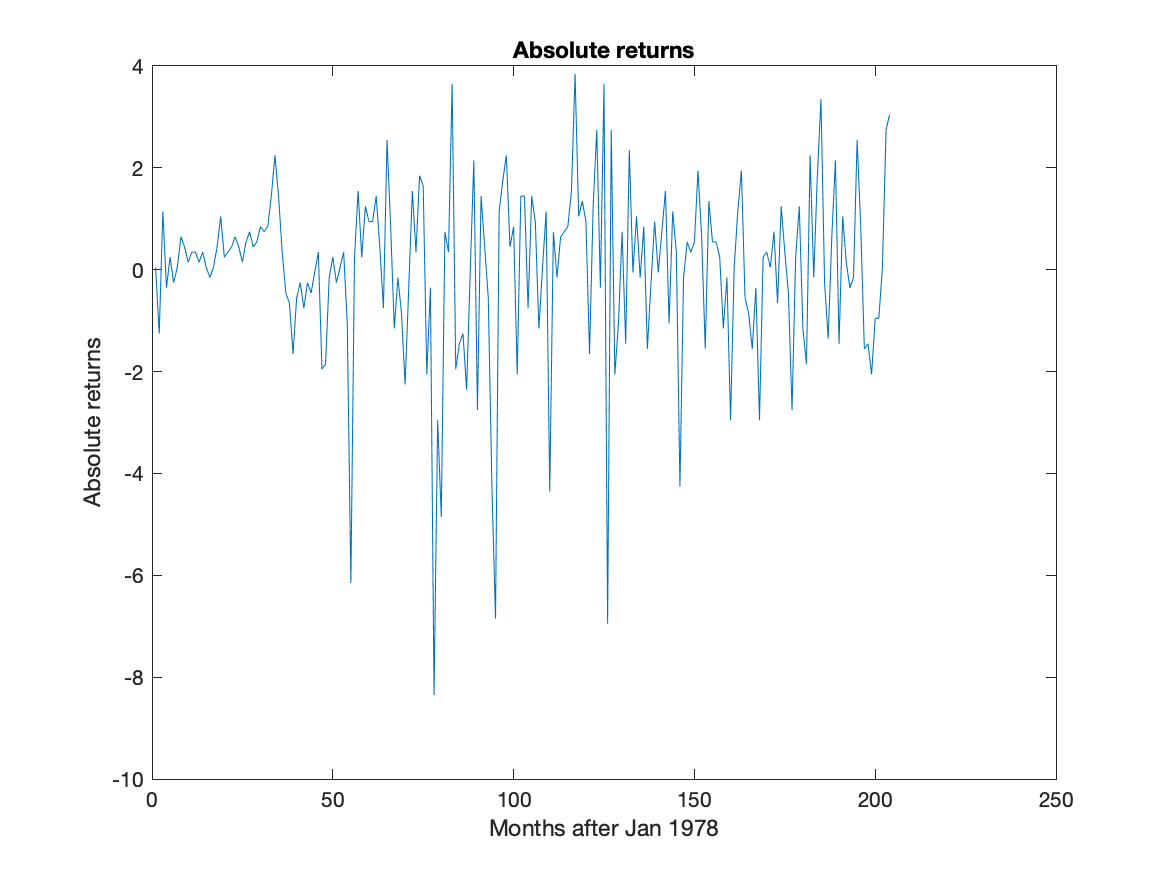
\includegraphics[width=10cm]{plots/abs_returns.png}
\centering
\caption{Absolute returns $Y_t = X_{t + 1} - X_{t}$}
\label{fig:absreturns}
\end{figure}

\begin{figure}[h!]
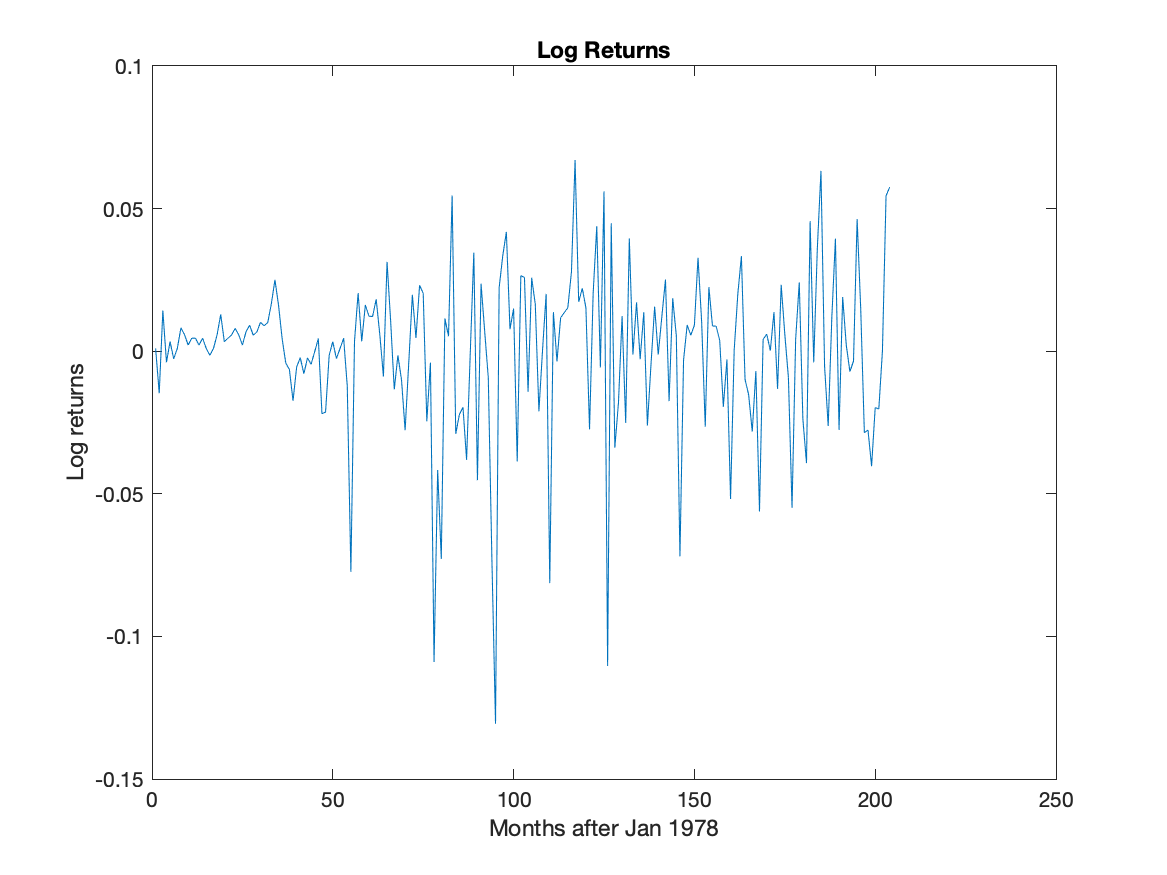
\includegraphics[width=10cm]{plots/log_returns.png}
\centering
\caption{Log returns $Z_t = \log(X_{t + 1}) - \log(X_{t})$}
\label{fig:logreturns}
\end{figure}

For both the absolute returns in Figure \ref{fig:absreturns} and the log returns in Figure \ref{fig:logreturns} it appears that the processes could be stationary.
There do not seem to be any pairs of points where the covariance of $X_{t + h}$ and $X_{t}$ would be dependent on the value of $t$.
The range of $t$ from $0 \leq t 40$ does appear slightly different from the rest of the series but not enough for us to think it would not be stationary.
Overall both series actually do not look like they have very much correlation at all between which could be an indication of independent and identically distributed time series.

\section*{Problem 2}
To test whether the series are iid or not we use the Ljung-Box test that compares the test statistic
$$
\lambda = n (n + 2) \sum_{i = 1}^h \frac{\hat{\rho}(i)^2}{n - i}
$$
Which has a $\chi^2_{h}$ distribution under the null hypothesis (that the data comes from and iid distribution
We want to test with $h = 20$ and $\alpha = 0.05$ so we compare $\lambda$ again the critical value, $\chi^2_{1-\alpha,h}$. That is, we reject the null hypothesis if
$$
\lambda > \chi^2_{.95,20} = 31.41
$$

For the standardized exchange rate data we found that $\lambda_1 = 3005$ which has a $p$-value of essentially 0. We can reject the null hypothesis and concluded that the exchange rate data is not iid.

For the absolute returns, we found that $\lambda_2 = 29.09$. That corresponds with a p-value of $0.086 > 0.05$. Here we fail to reject the null hypothesis (but we are fairly close to .05. There is some evidence to support the claim that the absolute returns come are iid.

The log returns have a test statistic $\lambda_3 = 23.19$ which has a p-value of 0.279. Here we fail to reject the null hypothesis as well which is consistent with the log returns being iid.

\section*{Problem 5}
\subsection*{Part a}
% Show expected value the same
\begin{align*}
    E[X_t] &= E[\cos(\omega t + Y)]\\
    &= E[\cos(\omega t) \cos(Y) - sin(\omega t) sin(Y)] && \text{Sum-difference for cos}\\
    &= \cos(\omega t) E[\cos(Y)] - sin(\omega t) E[sin(Y)]\\
    &= \text{TODO: Find dist. of cos(Y) and sin(Y)}
\end{align*}

\bibliographystyle{plain}
\bibliography{references}
\end{document}
